\documentclass[11pt,a4paper]{article}
\usepackage[T1]{fontenc}
\usepackage[margin=2.3cm]{geometry}
\usepackage{amsmath,amssymb}
\usepackage{graphicx}
\usepackage[dvipsnames]{xcolor}
\usepackage{enumitem}
\usepackage[colorlinks=true,linkcolor=blue,urlcolor=blue]{hyperref}
\setlength{\parskip}{0.6em}
\setlength{\parindent}{0pt}
\begin{document}

\begin{center}{\LARGE\bfseries openengine}\\[0.4em]{\large Compare Otto and Diesel engines on P-V diagrams, in three sessions.}\\[0.2em]\small PAN IIT OSS explainer \textbullet{} higher secondary to diploma / undergraduate (levels 4-5)\end{center}

\section*{Why this exists}
Every engine turns heat into work and rejects the rest. This explainer follows the idea from the energy balance to the Otto, Diesel and Carnot cycles and a numerical simulation, using only the gas laws and the first law of thermodynamics.

\section*{The end goal}
Compare Otto and Diesel cycle efficiency on P-V diagrams. The end goal is to compare Otto and Diesel cycle efficiency on P-V diagrams: to know what you hold equal, read the loops, and explain which engine wins and why. The same ideas apply to gas turbines, power plants and refrigerators.

\section*{How the three sessions build up}
\begin{enumerate}[nosep]
\item \textbf{Session 1: Heat in, work out, heat rejected} (Level 1, conceptual interactive model, 60 min).
\item \textbf{Session 2: Otto, Diesel and Carnot efficiency} (Level 2, mathematical engineering model, 75 min).
\item \textbf{Session 3: Simulate the cycle and validate it} (Level 3, simulation and validation, 90 min).
\end{enumerate}

\section{Session 1: Heat in, work out, heat rejected}

\subsection*{A. Real-world problem}
A car burns fuel, but most of the fuel's energy leaves through the exhaust and the radiator instead of turning the wheels. Why can no engine turn all the heat into work? And if you only see the pressure and volume of the gas inside the cylinder, how can you read off the work of one cycle? (General education only: this is a simplified model, not an engine design method.)

\subsection*{B. Concept and theory}
An engine takes heat Qh from a hot source, does work W and must throw heat Qc away to a cold place. After one full cycle the engine is back where it started, so its stored energy has not changed and the energy balance is Qh = W + Qc. The efficiency is the part of the heat that becomes work: eta = W / Qh. The second law says Qc cannot be zero; between a hot source at Th and cold surroundings at Tc (kelvin), no engine can beat eta = 1 - Tc / Th. On a graph of pressure against volume, expansion at high pressure gives more work than compression at low pressure takes back, so a clockwise loop gives net work and the work is the enclosed area. With P in kPa and V in litres, kPa times L equals joules.

\begin{itemize}[nosep]
\item Qh: heat taken from the hot source per cycle (J)
\item Qc: heat rejected to the cold surroundings per cycle (J)
\item W: net work per cycle (J)
\item eta: thermal efficiency W / Qh (no unit)
\item Th, Tc: hot and cold temperatures, absolute (K)
\item P, V: gas pressure and volume (kPa, L)
\end{itemize}

\begin{equation*}
Q_h = W + Q_c,\qquad W = Q_h - Q_c
\end{equation*}

\begin{equation*}
\eta = \frac{W}{Q_h} = 1 - \frac{Q_c}{Q_h}
\end{equation*}

\begin{equation*}
\eta \le \eta_{\mathrm{Carnot}} = 1 - \frac{T_c}{T_h}
\end{equation*}

\begin{equation*}
W = \oint P\,dV
\end{equation*}

\begin{center}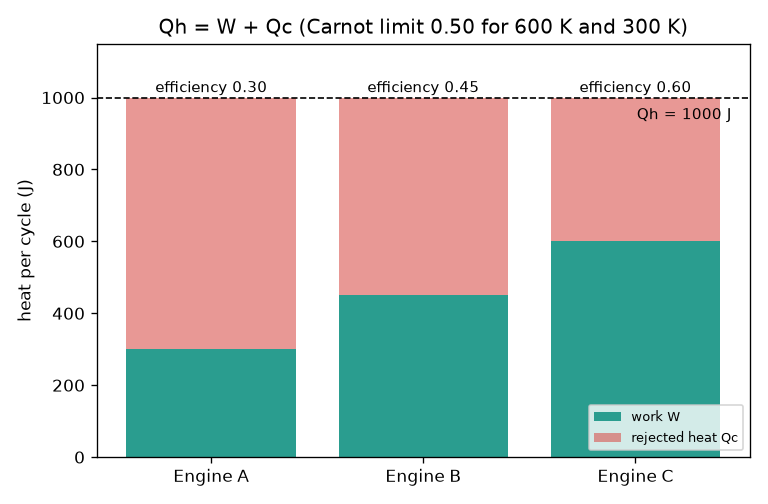
\includegraphics[width=0.85\linewidth]{figures/s01_energy_split.png}\\\small Three engines taking 1000 J: work and rejected heat; Engine C breaks the Carnot limit.\end{center}

\subsection*{E. Worked example}
An engine takes 1000 J from a 600 K source and rejects 650 J to 300 K surroundings. Find W and the efficiency and check the Carnot limit. Then find the work of a P-V rectangle from 100 to 300 kPa and 1 to 3 L.
\begin{enumerate}[nosep]
\item Energy balance: W = Qh - Qc = 1000 - 650 = 350 J.
\item Efficiency = 350 / 1000 = 0.35.
\item Carnot limit = 1 - 300 / 600 = 0.50; since 0.35 is below 0.50 the engine is allowed.
\item Loop area = (300 - 100) kPa x (3 - 1) L = 200 x 2 = 400 kPa L = 400 J.
\item If that loop were the same engine's cycle with Qh = 1000 J, then Qc = 600 J and eta = 0.40.
\end{enumerate}
\textbf{Answer.} W = 350 J, efficiency 0.35 (allowed, limit 0.50); the rectangle encloses 400 J.

\subsection*{F. Questions}
\begin{enumerate}[nosep]
\item \textbf{Conceptual.} Why can an engine never turn all of the heat it receives into work, even if it had no friction at all?
\item \textbf{Numerical.} An engine takes 800 J from a hot source and rejects 520 J. Find the work and the efficiency, and check the units and the answer is reasonable.
\item \textbf{Graph and simulation interpretation.} In the P-V view the loop is the same width but taller after you raise the work. By what factor does the area grow when the top pressure goes from 300 kPa to 500 kPa (bottom 100 kPa, volume 1 to 3 L)? What are the two works?
\item \textbf{Design and optimisation challenge.} Design: an engine must give 300 J of work per cycle between a 700 K source and 300 K surroundings. What is the smallest heat Qh it must take in, and the smallest Qc? A real engine reaches 0.30. How much heat would it need?
\end{enumerate}

\section{Session 2: Otto, Diesel and Carnot efficiency}

\subsection*{A. Real-world problem}
A petrol engine and a diesel engine both squeeze air, add heat and let the hot gas push a piston. What compression ratio do you need for an efficiency of 0.60, and why does a real engine, which is built to match such a cycle, reach much less? (Simplified air-standard model; not an engine design method.)

\subsection*{B. Concept and theory}
The air-standard model treats the working fluid as an ideal gas (P v = R T per kg) with constant gamma = cp / cv = 1.4, heated from outside and without friction or heat loss. The Otto cycle has four steps: isentropic compression 1 to 2 by the compression ratio r = V1 / V2, heat addition at constant volume 2 to 3, isentropic expansion 3 to 4, and heat rejection at constant volume 4 to 1. Along an isentrope T V\textasciicircum{}(gamma-1) and P V\textasciicircum{}gamma stay constant, which gives T2 = T1 r\textasciicircum{}(gamma-1) and the efficiency 1 - 1 / r\textasciicircum{}(gamma-1). The Diesel cycle adds heat at constant pressure, so the volume grows by the cut-off ratio rho = V3 / V2 during burning; its loss 1 - eta is the Otto loss times a factor that is above 1 for rho above 1, so at the same r its efficiency is lower. A larger r raises both, with diminishing returns. The Carnot limit 1 - Tc / Th uses the highest and lowest temperatures: Otto and Diesel add heat over a range of temperatures, not all at the peak, so they stay well below it. Real engines are lower again because of finite burn time, heat loss, friction, gas leakage and the change of gas properties with temperature; typically quoted brake efficiencies of petrol and diesel engines are roughly 25 to 40 percent (check a data sheet for a specific engine).

\begin{itemize}[nosep]
\item r: compression ratio V1 / V2 (no unit)
\item rho: cut-off ratio V3 / V2 (Diesel) (no unit)
\item gamma: cp / cv of the gas, 1.4 for air (no unit)
\item T1..T4: gas temperature at states 1 to 4 (K)
\item q\_in, q\_out: heat added, heat rejected (kJ/kg)
\item R, cv: gas constant 0.287 and R / (gamma - 1) = 0.7175 (kJ/(kg K))
\end{itemize}

\begin{equation*}
T_2 = T_1\, r^{\gamma-1},\qquad P V^{\gamma} = \mathrm{const}\ \text{(isentrope)}
\end{equation*}

\begin{equation*}
\eta_{\mathrm{Otto}} = 1 - \frac{1}{r^{\gamma-1}}
\end{equation*}

\begin{equation*}
\eta_{\mathrm{Diesel}} = 1 - \frac{1}{r^{\gamma-1}}\,\frac{\rho^{\gamma}-1}{\gamma(\rho-1)}
\end{equation*}

\begin{equation*}
\eta_{\mathrm{Carnot}} = 1 - \frac{T_c}{T_h}
\end{equation*}

\begin{equation*}
r = (1-\eta)^{-1/(\gamma-1)}\quad\text{(Otto design)}
\end{equation*}

\begin{center}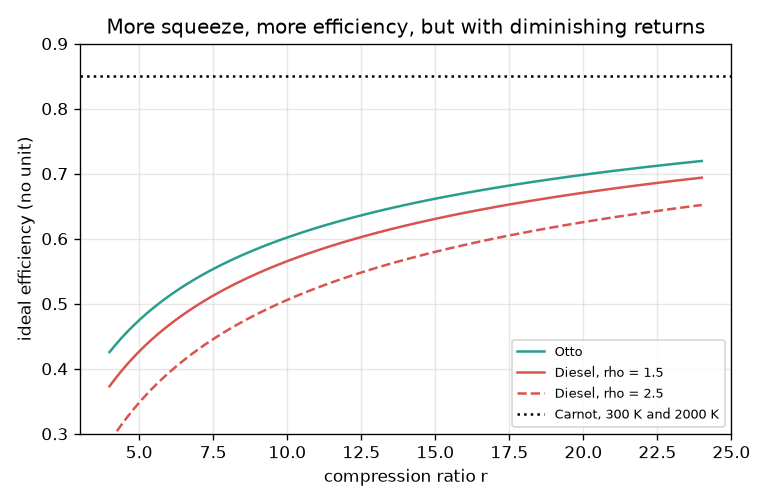
\includegraphics[width=0.85\linewidth]{figures/s02_eta_vs_r.png}\\\small Ideal efficiency against compression ratio for Otto, Diesel and the Carnot limit.\end{center}

\subsection*{E. Worked example}
An ideal Otto cycle with r = 9, gamma = 1.4, T1 = 300 K takes q\_in = 1100 kJ/kg. Find the temperatures, the efficiency from the heats, and compare with the formula and the Carnot limit.
\begin{enumerate}[nosep]
\item 9\textasciicircum{}0.4 = 2.408, so T2 = 300 x 2.408 = 722.5 K.
\item cv = 0.287 / 0.4 = 0.7175 kJ/(kg K). T3 = T2 + q\_in / cv = 722.5 + 1100 / 0.7175 = 2255.6 K.
\item T4 = T3 / 2.408 = 936.6 K. Heat rejected q\_out = cv (T4 - T1) = 0.7175 x 636.6 = 456.8 kJ/kg.
\item Efficiency from the heats = 1 - 456.8 / 1100 = 0.5848. Formula: 1 - 1 / 2.408 = 0.5847 (0.585). They agree.
\item Carnot between 300 K and 2255.6 K = 1 - 300 / 2255.6 = 0.867, much higher than 0.585, because heat is added from 722 K upward, not all at 2256 K.
\end{enumerate}
\textbf{Answer.} T2 = 722.5 K, T3 = 2255.6 K, T4 = 936.6 K; efficiency 0.585 (Otto) against a Carnot limit of 0.867.

\subsection*{F. Questions}
\begin{enumerate}[nosep]
\item \textbf{Conceptual.} At the same compression ratio and the same heat input, which is more efficient, Otto or Diesel, and why?
\item \textbf{Numerical.} Find the ideal Otto efficiency for r = 8 and gamma = 1.4, and for the Diesel at r = 18 with rho = 2. Show the working.
\item \textbf{Graph and simulation interpretation.} From the efficiency graph, is it worth raising r from 19 to 20? Compare with raising it from 9 to 10.
\item \textbf{Design and optimisation challenge.} Design: choose r so that an ideal Otto engine reaches 0.60. A Diesel with r = 18 must also reach 0.60: what is the largest cut-off ratio allowed? Why will the real engines still be well below 0.60?
\end{enumerate}

\section{Session 3: Simulate the cycle and validate it}

\subsection*{A. Real-world problem}
The formulas of Session 2 assume that heat arrives instantly and that nothing is lost. A real engine burns fuel over tens of crank degrees, loses heat to its walls and drags against friction. Can we simulate the cycle step by step, show that it reproduces the formulas when we switch the real effects off, measure how much each effect costs, and choose a compression ratio for a small generator engine? (A simplified teaching model, not a design tool.)

\subsection*{B. Concept and theory}
For a small step of a closed ideal gas the first law is dQ = dU + P dv with U = P v / (gamma - 1) per kg. This gives dP/dv = -gamma P / v with no heat (integrated with Runge-Kutta 4), dP = (gamma - 1) dQ / v at constant volume and dv = (gamma - 1) dQ / (gamma P) at constant pressure. The work is the sum of P dv around the closed loop (trapezoid rule), and the first law demands net work = q\_in - q\_out. A crank-angle model uses the slider-crank volume V(a) and releases heat along a Wiebe curve x = 1 - exp(-A z\textasciicircum{}(m+1)), z = (a - a0) / duration, with A = 6.908 and m = 2; the pressure obeys dP/da = ((gamma - 1) dQ/da - gamma P dV/da) / V. A share of the heat can be lost to the walls, and friction is subtracted as a friction mean effective pressure times the displacement. Two fair comparisons: at equal compression ratio and heat Otto wins, but at equal peak pressure (the structural limit) the Diesel can compress harder before burning and wins. Knock: in a spark-ignition engine the unburnt end gas, heated to about T1 r\textasciicircum{}(gamma-1), can ignite by itself, causing a damaging pressure shock; this sets an upper limit on r for a given fuel. A diesel compresses only air and injects fuel at the end, so it avoids this particular limit.

\begin{itemize}[nosep]
\item v, P: specific volume and pressure of the gas (m3/kg, kPa)
\item q\_in: heat added per kg of air (kJ/kg)
\item a: crank angle from top dead centre (degrees)
\item loss: share of heat lost to the walls (no unit)
\item fmep: friction mean effective pressure (kPa)
\item T2: end-of-compression air temperature (K)
\end{itemize}

\begin{equation*}
dQ = dU + P\,dv,\quad U = \frac{P v}{\gamma-1}
\end{equation*}

\begin{equation*}
\frac{dP}{dv} = -\gamma\frac{P}{v}\ \text{(no heat)}
\end{equation*}

\begin{equation*}
\frac{dP}{da} = \frac{(\gamma-1)\,dQ/da - \gamma P\,dV/da}{V}
\end{equation*}

\begin{equation*}
x_b(a) = 1 - \exp\!\left[-A\left(\frac{a-a_0}{\Delta a}\right)^{m+1}\right]
\end{equation*}

\begin{equation*}
W = \oint P\,dv \approx \sum \tfrac12 (P_i + P_{i+1})(v_{i+1} - v_i),\qquad W = q_{\mathrm{in}} - q_{\mathrm{out}}
\end{equation*}

\begin{center}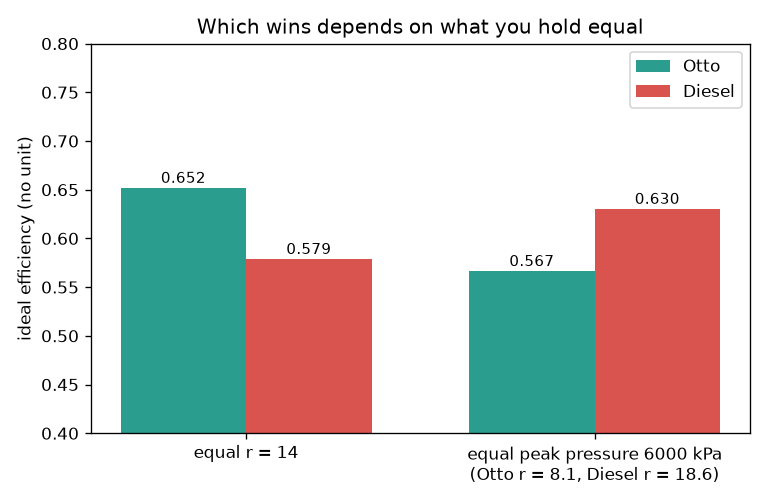
\includegraphics[width=0.85\linewidth]{figures/s03_fair_comparison.png}\\\small Otto beats Diesel at equal compression ratio; Diesel beats Otto at equal peak pressure.\end{center}

\subsection*{E. Worked example}
Simulate the ideal Otto cycle with r = 9 and q\_in = 1100 kJ/kg (P1 = 100 kPa, T1 = 300 K). Compare its efficiency with the formula and check the first law.
\begin{enumerate}[nosep]
\item Compression: integrate dP/dv = -gamma P / v from v1 = 0.861 to v2 = 0.0957 m3/kg in 400 steps.
\item Heat at constant volume: add 1100 kJ/kg in 400 equal steps, dP = 0.4 dQ / v2; then expand back to v1 and cool to P1 at constant volume.
\item Sum P dv around the loop: net work = 643.3 kJ/kg; heat rejected = v1 (P4 - P1) / 0.4 = 456.8 kJ/kg.
\item Efficiency = 643.3 / 1100 = 0.58477; the formula gives 0.58476.
\item First law: net work - (q\_in - q\_out) = 0.02 kJ/kg, about 0.002 percent of the heat input.
\end{enumerate}
\textbf{Answer.} Simulated efficiency 0.5848 (formula 0.5848), net work 643 kJ/kg, rejected heat 457 kJ/kg, first-law error 0.02 kJ/kg.

\subsection*{F. Questions}
\begin{enumerate}[nosep]
\item \textbf{Conceptual.} Why does a Diesel win at equal peak pressure although an Otto wins at equal compression ratio?
\item \textbf{Numerical.} Find the end-of-compression temperature for r = 10 and r = 9 (T1 = 300 K, gamma = 1.4). A fuel allows T2 up to 740 K with a 20 K margin: is r = 10 acceptable?
\item \textbf{Graph and simulation interpretation.} In the knock-down figure, which single real effect costs the most efficiency, and by how much? Compare the burn time, the heat loss and the friction.
\item \textbf{Design and optimisation challenge.} Design: a generator engine uses fuel A (T2 limit 740 K) with a 20 K margin, or fuel B (800 K). Choose r for each in steps of 0.5, find the modelled brake efficiency (10 percent loss, friction 100 kPa) and say which fuel meets a 0.45 target. What r would be needed?
\end{enumerate}

\section{Real-world mini-project}
\textbf{Choose the compression ratio of a small generator engine.} A small generator engine can run on fuel A or fuel B. For illustration, fuel A tolerates an end-of-compression air temperature T2 of 740 K before it knocks and fuel B tolerates 800 K; the designer keeps a margin of 20 K. Use \texttt{max\_r\_knock\_free} and \texttt{engine\_cycle} from Session 3 (heat 1100 kJ/kg of air, Wiebe burn of 40 degrees from -10, 10 percent heat loss, friction mean effective pressure 100 kPa). The owner wants a brake efficiency of at least 0.45. These limits are illustrative numbers, not fuel specifications.

\section{The path ahead}
\begin{enumerate}[nosep]
\item \textbf{Session 4: Temperature-dependent gas properties.} The Otto cycle with cv(T) from a simple polynomial instead of a constant gamma.
\item \textbf{Session 5: The dual (Seiliger) cycle.} A function that splits the heat and returns efficiency and a P-V path.
\item \textbf{Session 6: T-S diagram from the simulation.} Compute entropy along the simulated cycle and draw the T-S loop with the Carnot rectangle.
\item \textbf{Session 7: A knock model with engine speed.} An induction-time integral on the end-gas temperature history.
\item \textbf{Session 8: Four strokes with a pumping loop.} Add gas exchange to the crank-angle model with a throttled intake.
\end{enumerate}

\section{Answers and hints}

\subsection*{Session 1}
\begin{enumerate}[nosep]
\item \textbf{Conceptual.} Hint: What does the second law say about Qc, and what would eta = 1 - Tc / Th need? Solution: The second law forbids a cyclic engine that takes heat from one source and turns all of it into work. Some heat Qc must go to a colder place. The best case is the Carnot limit 1 - Tc / Th, which reaches 1 only if Tc were 0 K (or Th infinite), and neither is possible. So even a frictionless engine has an efficiency below 1.
\item \textbf{Numerical.} Hint: W = Qh - Qc, then divide by Qh. Solution: W = 800 - 520 = 280 J. eta = 280 / 800 = 0.35 (no unit). Sanity check: the efficiency is between 0 and 1, and W plus Qc gives back 800 J.
\item \textbf{Graph and simulation interpretation.} Hint: Area = (top - bottom) x width. Solution: The heights are 200 kPa and 400 kPa, so the area doubles: 400 J becomes 800 J (units: kPa L = J).
\item \textbf{Design and optimisation challenge.} Hint: Use the Carnot limit as the best case: Qh = W / eta. Solution: Best case eta = 1 - 300 / 700 = 0.571, so Qh = 300 / 0.571 = 525 J and Qc = 225 J. A real engine at 0.30 needs Qh = 300 / 0.30 = 1000 J and rejects 700 J. Trade-off: the Carnot value is a floor on the heat you must supply, not a design target, because real engines are far below it.
\end{enumerate}

\subsection*{Session 2}
\begin{enumerate}[nosep]
\item \textbf{Conceptual.} Hint: Where in the piston stroke is the heat added in each cycle? Solution: Otto. Its heat is added at constant volume while the piston is at the top, so all of it is expanded through the full stroke. The Diesel adds part of its heat while the piston is already moving down, so that heat is expanded less. The factor (rho\textasciicircum{}gamma - 1) / (gamma (rho - 1)) is above 1, which lowers the Diesel efficiency.
\item \textbf{Numerical.} Hint: Use 8\textasciicircum{}0.4 and 18\textasciicircum{}0.4, and 2\textasciicircum{}1.4 = 2.639. Solution: Otto: 8\textasciicircum{}0.4 = 2.297, so eta = 1 - 1 / 2.297 = 0.565. Diesel: 18\textasciicircum{}0.4 = 3.178, so 1 / 3.178 = 0.3147; factor = (2.639 - 1) / (1.4 x 1) = 1.171; eta = 1 - 0.3148 x 1.171 = 0.632. Both are between 0 and 1 and below the Otto value at r = 18 (0.685), as expected.
\item \textbf{Graph and simulation interpretation.} Hint: Read how steep each curve is at those r values. Solution: The curves flatten. From 9 to 10 the Otto efficiency gains 0.017; from 19 to 20 only 0.006, about a third as much, while the cost (peak pressure, knock, strength) rises. So the same extra squeeze buys much less at high r.
\item \textbf{Design and optimisation challenge.} Hint: Invert: r = (1 - eta)\textasciicircum{}(-1/0.4); for the Diesel solve the formula for rho numerically. Solution: Otto: r = 0.4\textasciicircum{}(-2.5) = 9.88, about 10. Diesel at r = 18: the largest rho is 2.73 (above that eta drops below 0.60); in heat terms this limits how much fuel can burn at constant pressure. Real engines are lower because the burn takes time, heat leaks to the walls, friction takes work, and the gas properties change at high temperature (gamma falls); the model also ignores gas exchange. Constraint: higher r raises pressure, structural load and (for petrol) the risk of knock, treated in Session 3.
\end{enumerate}

\subsection*{Session 3}
\begin{enumerate}[nosep]
\item \textbf{Conceptual.} Hint: What limits each engine: the compression ratio or the peak pressure? Solution: At equal r the comparison favours the Otto because all its heat is added at top dead centre. But strength limits the peak pressure, not r. The Otto's peak pressure comes after heat addition at constant volume, so it must keep r low (8.1 for 6000 kPa); the Diesel's peak pressure is the end of compression, so it can use r = 18.6 and the higher r wins (0.63 against 0.57).
\item \textbf{Numerical.} Hint: T2 = T1 r\textasciicircum{}0.4; margin means T2 must not exceed 720 K. Solution: r = 10: 10\textasciicircum{}0.4 = 2.512, so T2 = 300 x 2.512 = 754 K. r = 9: 9\textasciicircum{}0.4 = 2.408, so T2 = 722 K. The allowed value is 740 - 20 = 720 K, so r = 10 is not acceptable and even r = 9 (722 K) is just too hot; the largest allowed r in steps of 0.5 is 8.5 (T2 = 706 K).
\item \textbf{Graph and simulation interpretation.} Hint: Take differences between the neighbouring bars: 0.584, 0.570, 0.513, 0.443. Solution: Burn time costs 0.584 - 0.570 = 0.014, 10 percent heat loss costs 0.570 - 0.513 = 0.057 and friction of 100 kPa costs 0.513 - 0.443 = 0.070. Friction costs the most in this setting, then heat loss; the finite burn is the smallest. (The numbers depend on the illustrative values.)
\item \textbf{Design and optimisation challenge.} Hint: Use max\_r\_knock\_free and engine\_cycle. Solution: Fuel A: r = 8.5 (T2 = 706 K), brake 0.436: misses the target. Fuel B: r = 10.5 (T2 = 768 K), brake 0.463: meets it. The smallest r that reaches 0.45 is 9.5 (T2 = 738 K), which fuel A cannot allow with its margin. Trade-off: a better fuel (or a lower friction or loss) is needed for the target; raising r above the knock limit would risk damage. All limits are illustrative.
\end{enumerate}

\section{How to join}
Read \texttt{CONTRIBUTING.md} in the repository, then pick an issue labelled \texttt{good first issue}. Repository: \url{https://github.com/KrunalPanchal1995/openengine}

\end{document}
